\chapter{Graphs and Trees}

In this chapter there are many exemples of using nodes and paths to draw diagrams.

\begin{figure}[hbt]
    \centering
   \begin{tikzpicture}
\node (shape) at (0,2) [draw] {class Shape};
\node (rect) at (-2,0) [draw] {class Rectangle};
\node (circle) at (2,0) [draw] {class Circle};
\node (ellipse) at (6,0) [draw] {class Ellipse};

\draw (node cs:name=ellipse,anchor=north) |- (0,1);
\draw (node cs:name=circle,anchor=north)
  |- (0,1);

\draw [arrows = -{Triangle[open, angle=60:3mm]}]
(node cs:name=rect,anchor=north) |- (0,1) -| (node cs:name=shape,anchor=south);
\end{tikzpicture}
    \caption{Caption}
    \label{fig:my_1label}
\end{figure}


\begin{figure}
    \centering
\begin{tikzpicture}[shorten >=1pt,node distance=2cm,on grid]
\node[state,initial] (q_0) {$q_0$};
\node[state] (q_1) [right=of q_0] {$q_1$};
\node[state](q_2) [right=of q_1] {$q_2$};
\node[state,accepting](q_3) [right=of q_2] {$q_3$};
\path[->] (q_0) edge node [above] {0} (q_1)
edge [loop above] node {1} ()
edge [bend left] node [above] {2} (q_2)
edge [bend right] node [below] {3} (q_3)
(q_1) edge node [above] {4} (q_2);
\path[->] (q_2) edge node [above] {5} (q_3);
\end{tikzpicture}
    \caption{Based on the   topathas manual.}

\end{figure}


\begin{figure}
    \centering
    \begin{tikzpicture}
[every node/.style={node distance=1cm and 0.3cm}]
\node (St1) at (0,0) {\{stock, broth\}};
\node (St2) [right  =  of St1] {\{stock, breed\}};
\node (St3) [right = of St2] {\{stock, share\}};
\node (D) [above = of St1] {\{soup\}};
\node (V) [above = of St2] {\{variety\}};
\node (A) [above = of St3] {\{asset\}};
\node (B) [below = of St1] {\{beef broth, beef stock\}};

\draw[-Latex] (St1) -- node [midway,right] {\tiny is-a} (D);
\draw[-Latex] (St2) -- node [midway,right] {\tiny is-a} (V);
\draw[-Latex] (St3) -- node [midway,right] {\tiny is-a} (A);
\draw[-Latex] (St1) -- node [midway,right] {\tiny like-a} (B);
\draw[-Latex] ([xshift=2em]B.north west) -- node [midway,right] {\tiny is-a} ([xshift=-2em]St1.south);
\end{tikzpicture}
    \caption{Relations from Wordnet}
    \label{fig:wordnet1}
\end{figure}

\begin{figure}
    \centering
    \begin{tikzpicture}
    \useasboundingbox (1,-3) rectangle (5,4);
    \scope[transform canvas={scale=.6}]
         % Your actual drawing

    \begin{scope}
        [
            grow=right,
            level 1/.style={sibling distance=18em,level distance=2.5cm},
            level 2/.style={sibling distance=14em,level distance=4.5cm}
            ,
            every node/.style =
            {   shape=rectangle, rounded corners,
                draw, align=center,
                fill=white,
                font=\Large,
                inner sep=5pt % espaço entre texto e borda
            },
            every annotation/.style={rectangle,
            rounded corners=0mm,
            font=\normalsize}
        ]
  \node (inc) {Incerteza} % root
    child { node {Nebulosidade}
        child { node[annotation]
                {Faltam distinções precisas ou definidas
                \begin{itemize}\setlength\itemsep{0em}
                    \item Vago
                    \item Confuso
                    \item Falta de Clareza
                    \item Indistinto
                    \item Impreciso
                \end{itemize}
                }
        }
    }
    child { node (amb) {Ambiguidade}
    child { node {Discordância}
         child { node[annotation]
                {Desacordo ao escolher uma alternativa
                 \begin{itemize}\setlength\itemsep{0em}
                    \item Dissonância
                    \item Incongruência
                    \item Discrepância
                    \item Conflito
                \end{itemize}
                }
        }
    }
    child { node {Não-especificidade}
    child { node[annotation]
                {Alternativas não especificadas
                 \begin{itemize}\setlength\itemsep{0em}
                    \item Variedade
                    \item Generalidade
                    \item Diversividade
                    \item Equívoco
                    \item Imprecisão
                \end{itemize}
                }
        }
    }
    };
    \end{scope}

      \begin{scope}[every annotation/.style={fill=gray!20,text=black}]
      \node [annotation,above left] at (amb.north)
{relacionamentos 1 para muitos};
\end{scope}
    \endscope
\end{tikzpicture}
    \caption{Exemplo de uso de Transform Canvas, mas que não deu certo no documento em que foi usado, pois gerou outras mudanças}

\end{figure}


\begin{figure}[hbt]
\centering
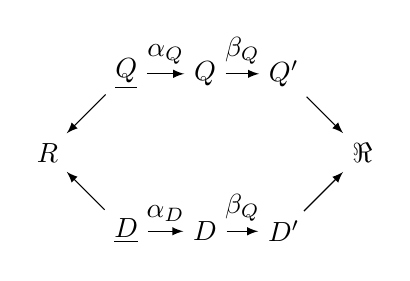
\begin{tikzpicture}
    \tikzmath{  \x1 = 0 ;
                \x5 = 8 ;
                \y1 = 0 ;
                \y2 = 1 ;
                \y3 = 2 ;
                \x3 = \x5 /2 ;
                \x2 = \x3 /2;
                \x4 = (\x3+\x5)/2;
                }

\node (R) at (\x1,\y2) {$R$};
\node (Q1) at (\x2,\y3) {$\underline{Q}$};
\node (D1) at (\x2,\y1) {$\underline{D}$};
\node (Q2) at (\x3,\y3) {$Q$};
\node (D2) at (\x3,\y1) {$D$};
\node (Q3) at (\x4,\y3) {$Q^\prime$};
\node (D3) at (\x4,\y1) {$D^\prime$};
\node (VSR) at (\x5,\y2) {$\Re$};

\draw[-latex] (Q1) -- (R) ;
\draw[-latex] (D1) -- (R) ;
\draw[-latex] (Q1) -- (Q2) node[midway,above] {$\alpha_Q$};
\draw[-latex] (D1) -- (D2)
node[midway,above] {$\alpha_D$};
\draw[-latex] (Q2) -- (Q3) node[midway,above] {$\beta_Q$};
\draw[-latex] (D2) -- (D3)
node[midway,above] {$\beta_Q$};
\draw[-latex] (Q3) -- (VSR);
\draw[-latex] (D3) -- (VSR);
\end{tikzpicture}
\caption{Figure from IR, first try, using calculated absolute positions}
\label{fig:ir}
\end{figure}

\begin{figure}[hbt]
\centering
\begin{tikzpicture}
\node (R) at (0,0) {$R$};
\node (Q1) [above right = of R] {$\underline{Q}$};
\node (D1) [below right = of R] {$\underline{D}$};
\node (Q2) [right = of Q1] {$Q$};
\node (D2) [right = of D1]  {$D$};
\node (Q3) [right = of Q2]  {$Q^\prime$};
\node (D3) [right = of D2]  {$D^\prime$};
\node (VSR) [below right = of Q3] {$\Re$};

\draw[-latex] (Q1) -- (R) ;
\draw[-latex] (D1) -- (R) ;
\draw[-latex] (Q1) -- (Q2) node[midway,above] {$\alpha_Q$};
\draw[-latex] (D1) -- (D2)
node[midway,above] {$\alpha_D$};
\draw[-latex] (Q2) -- (Q3) node[midway,above] {$\beta_Q$};
\draw[-latex] (D2) -- (D3)
node[midway,above] {$\beta_Q$};
\draw[-latex] (Q3) -- (VSR);
\draw[-latex] (D3) -- (VSR);
\end{tikzpicture}
\caption{Figure from IR, second try, using relative positions.}
\label{fig:ir2}
\end{figure}




\begin{figure}
    \centering
\begin{tikzpicture}[
  tlabel/.style={pos=0.4,right=-1pt,font=\footnotesize\color{red!70!black}},
]
\node{S}
child {node {a}}
child {node {S}
  child {node {a}}
  child {node {S}
    child {node {$\varepsilon$}
      edge from parent node[tlabel,pos=0.2] {2}
    }
    edge from parent node[tlabel] {1}
  }
  child {node {B}
    child {node {B}
      child {node {b}
        edge from parent node[tlabel,pos=0.2] {5}
     }
      edge from parent node[tlabel] {4}
    }
    child {node {b}}
  }
    edge from parent node[tlabel] {1}
  }
child {node {B}
  child[missing] {}
  child[missing] {}
  child {node {b}
    edge from parent node[tlabel,pos=0.15,right=2pt] {5}
  }
};
\end{tikzpicture}    \caption{This tree is described in https://tex.stackexchange.com/questions/85112/drawing-a-syntax-tree-in-tikz}
    \label{fig:my_2label}
\end{figure}


\begin{figure}
centering
\resizebox{0.8\textwidth}{!}{
\begin{tikzpicture}[
  ->,
  >=stealth',
  edge from parent/.style={thick,draw=black!70,-latex},
  level 1/.style={sibling distance=8.5cm},
  level 2/.style={child anchor=north},
  level 3/.style={child anchor=north,sibling distance=2cm},
  level distance=3.5cm,
  auto,
  tree nodes/.style={
    shape=rectangle,
    rounded corners,
    thick,
    draw=black!75,
    minimum size=+5mm
  },
  and/.style     ={tree nodes, top color=blue!10, bottom color=white},
  or/.style      ={tree nodes, top color=red!10,  bottom color=white},
  terminal/.style={tree nodes, top color=green!5, bottom color=white},
  relation/.style={tree nodes, inner sep=2pt, fill=gray!20, font=\scriptsize},
  font=\footnotesize,
  every node/.append style={align=center}
]
\node              [and]                     {1 \\ 2 \\ 3}
  child {     node [and]      (appr)         {1 \\ 2 \\ 3}
    [sibling distance = 2cm]
    child {   node [terminal] (car)          {2}          }
    child {   node [relation] (rel)          {1 \\ 2 \\ 3}}
    child {   node [terminal] (zebra)        {1 \\ 2 \\ 3}}
  }
  child {     node [or]       (obstacle)     {1 \\ 2 \\ 3}
    [sibling distance = 6cm]
    child {   node [and]      (ped_on_zebra) {1 \\ 2 \\ 3}
      child { node [terminal] (ped)          {1}          }
      child { node [relation] (rel_1)        {1 \\ 2 \\ 3}}
      child { node [terminal] (zebra_2)      {1 \\ 2 \\ 3}}
    }
    child   { node [and]      (dog_on_zebra) {1 \\ 2 \\ 3}
      child { node [terminal] (dog)          {3}          }
      child { node [relation] (rel_2)        {1 \\ 2 \\ 3}}
      child { node [terminal] (zebra_1)      {1 \\ 2 \\ 3}}
    }
  };

\path [dashed,-]
  (rel) edge (zebra)
        edge (car)

  (rel_1) edge (ped)
          edge (zebra_2)

  (rel_2) edge (dog)
          edge (zebra_1);

\begin{scope}[shift={(7,1)}, node distance=+1cm, on grid, label position=right, start chain=ch going above]
  \foreach \sStyle/\tText in {relation/Relation, terminal/Terminal-Node, and/And-Node, or/Or-Node}
    \node[
     on chain=ch,
     \sStyle,
     label={= \tText}
    ] {};
\end{scope}
\end{tikzpicture}}
\caption{This tree is described in \url{https://tex.stackexchange.com/questions/123212/tikz-tree-some-childs-without-arrows}}
    \label{fig:my_3label}
\end{figure}

\begin{figure}[hbt]
\centering
\begin{tikzpicture}
\node {S}
    child {node {SN}
        child {node {Det$_m$}
            child {node {\textit{O}}}
        }
        child {node {N$_M$}
            child {node {\textit{menino}}}
        }
    }
    child {node[xshift=2cm] {SV}
    %child {node {}}
        child {node {SV}
            child {node {V$_t$}
                child {node {viu}}
            }
            child {node {SN}
                child {node {Det$_f$}
                    child {node {\textit{a}}}
                }
                child {node {N$_f$}
                    child {node {\textit{mulher}}}
                }
            }
        }
        child {node {SP}
            child {node[xshift=2cm] {P}
                child {node{com}
            }
            child {node {SN}
                child {node {Det$_m$}
                    child {node {o}
                    }
                }
                child {node {N$_m$}
                    child {node {binóculo}
                    }
                }
            }
        }
    }
};
\end{tikzpicture}
\caption{Primeira forma de interpretar sintaticamente a sentença ``O menino viu a mulher de binóculo'', onde o menino tem o binóculo, baseado em ...}
\label{fig:a1}
\end{figure}

\begin{figure}[hbt]
\centering
\begin{tikzpicture}
\node {S}
    child {node {SN}
        child {node {Det$_m$}
            child {node {\textit{O}}}
        }
        child {node {N$_M$}
            child {node {\textit{menino}}}
        }
    }
    child {node[xshift=1cm] {SV}
        child {node {V$_t$}
            child {node {viu}
            }
        }
        child {node {SN}
            child {node {Det$_f$}
                child {node {\textit{a}}
                }
            }
            child {node {N'$_f$}
                child {node {N$_f$}
                    child {node {\textit{mulher}}
                    }
                child {node {SP}
                    child {node {P}
                        child {node{com}
                        }
                    }
                    child {node[xshift=.5cm] {SN}
                        child {node {Det$_m$}
                            child {node {o}
                            }
                        }
                        child {node {N$_m$}
                            child {node {binóculo}
                            }
                        }
                    }
                }
            }
        }
    }
};
\end{tikzpicture}
\caption{Segunda forma de interpretar sintaticamente a sentença ``O menino viu a mulher de binóculo'', onde a mulher tem o binóculo, baseado em ...}
\label{fig:a2}
\end{figure}

\begin{figure}
    \centering
\begin{tikzpicture}
\begin{scope}
  \tikzset{edge from parent/.append style={draw=none},
  every tree node/.style={draw=none},level distance=2cm
  }
  \Tree [[.{Level 1} [.{Level 2} ]]]
\end{scope}
  \begin{scope}[xshift=2in]
\tikzset{every tree node/.style={draw,circle, minimum size=2em,fill=blech},
    level distance=2cm,sibling distance=1cm}
    \Tree[.\node (Root) {};
       [.4 11 {} ]
       [.5 6  {} ]
       ]
   \node [above=.25cm of Root] {Root};
\end{scope}
\end{tikzpicture}    \caption{https://tex.stackexchange.com/questions/153598/how-to-draw-empty-nodes-in-tikz-qtree}

\end{figure}


\begin{figure}
    \centering
\begin{tikzpicture}
[every node/.style={node distance=1cm and 0.3cm}]
\node (C) at (0,0) {\{Communicate\}};
\node (T) [below = of C] {\{talk\}};
\node (S) [below right = of T] {\{stammer\}};
\node (W) [below left = of T] {\{whisper\}};

\draw[-Latex] (C) -- (T);
\draw[-Latex] (T) -- (S);
\draw[-Latex] (T) -- (W);
\end{tikzpicture}

\begin{tikzpicture}
[every node/.style={node distance=1cm and 0.3cm}]
\node (C) at (0,0) {\{car\}};
\node (T) [below = of C] {\{engine\}};
\node (S) [below right = of T] {\{spark plug\}};
\node (W) [below left = of T] {\{cylinder\}};

\draw[Latex-] (C) -- node [midway,right] {\tiny is-part-of} (T);
\draw[Latex-] (T) -- node [midway,right] {\tiny is-part-of}(S);
\draw[Latex-] (T) -- node [midway,right] {\tiny is-part-of} (W);
\end{tikzpicture}
    \caption{Wordnet}
    \label{fig:wordnet2}
\end{figure}

\begin{figure}
    \centering
    \begin{tikzpicture}
\begin{scope}[
every node/.style = {node distance={10mm},
shape=rectangle, rounded corners,
                draw, align=center,
                fill=white,
                font=\Large,
                inner sep=8pt }
]
\node (NB) {\textbf{Nota Baixa}};
\node (PD) [below left = of NB] {\textbf{Prova Difícil}};
\node (NFLE) [right = of PD] {\textbf{Não Fiz Lista de Exercícios}};
\draw[-{Latex[length=3mm]}] (PD) -- (NB.south west);
\draw[-{Latex[length=3mm]}] (NFLE) -- (NB.south east);
\node (NE) [below = of PD] {\textbf{Não Estudei}} ;
\draw[-{Latex[length=3mm]}] (NE) -- (PD);
\node (NTT)  [below right = of NE] {\textbf{Não Tive Tempo}};
\draw[-{Latex[length=3mm]}] (NTT) -- (NE.south east);
\draw[-{Latex[length=3mm]}] (NTT) -- (NFLE);
\node (NMO)  [below  = of NTT,fill = yellow] {\textbf{Não Me Organizei}};
\draw[-{Latex[length=3mm]}] (NMO) -- (NTT);
\end{scope}
 \end{tikzpicture}
    \caption{Grafo - Diagrama de Causas Raiz Vertical}
    \label{fig:my_label12312}
\end{figure}

\begin{figure}
    \centering
  \begin{tikzpicture}
    \graph[spring layout] {
      A -> ["1"] B,
      A -> {C, D},
      C -> {B, D},
    };
  \end{tikzpicture}
    \caption{Auto layout}
    \label{fig:my_label5492}
\end{figure}


\section{Nodes With Lists Inside}

\begin{figure}
    \centering

    \begin{tikzpicture}
    \begin{scope}
        [->,>=stealth',
            grow=down,
            level 1/.style={sibling distance=12em,level distance=2cm},
            level 2/.style={sibling distance=12em,level distance=2cm,shorten >=0cm},
            level 3/.style={sibling distance=10em,level distance=2cm,shorten >=0cm},
            every node/.style =
            {   shape=rectangle,
                rounded corners,
                draw,
                align=center,
                fill=white,
                font=\large,
                inner sep=5pt % espaço entre texto e borda
            },
            every annotation/.style={shape=rectangle,
            rounded corners=0mm,
            font=\footnotesize}
        ]
  \node (inc) {\textbf{Incerteza}} % root
    child { node {Nebulosidade}
        child { node[annotation,align=left]
                {Faltam distinções precisas ou definidas
                \begin{itemize}\setlength\itemsep{-.5em}
                    \item Vago
                    \item Confuso
                    \item Falta de Clareza
                    \item Indistinto
                    \item Impreciso
                \end{itemize}
                }
        }
    }
    child { node (amb) {Ambiguidade}
    child { node[yshift=-2cm] {Discordância}
         child { node[annotation,align=left]
                {Desacordo ao escolher uma alternativa
                 \begin{itemize}\setlength\itemsep{-.5em}
                    \item Dissonância
                    \item Incongruência
                    \item Discrepância
                    \item Conflito
                \end{itemize}
                }
        }
    }
    child { node {Não-especificidade}
    child { node[annotation,align=left]
                {Alternativas não especificadas
                 \begin{itemize}\setlength\itemsep{-.5em}
                    \item Variedade
                    \item Generalidade
                    \item Diversividade
                    \item Equívoco
                    \item Imprecisão
                \end{itemize}
                }
        }
    }
    };
    \end{scope}

      \begin{scope}[every annotation/.style={fill=gray!20,text=black}]
      \node [annotation,above right ,align=center,text width=2cm] at (amb.north)
{relacionamentos \\ 1 para muitos};
\end{scope}

\end{tikzpicture}




    \caption{Graph Tree}



\end{figure}

\begin{figure}
    \centering
    \begin{tikzpicture}
    \begin{scope}
        [   ->,
            grow=right,
            level 1/.style={sibling distance=12em,level distance=.7cm},
            level 2/.style={sibling distance=10em,level distance=4cm,}
            ,
            every node/.style =
            {   shape=rectangle,
                rounded corners,
                draw,
                align=center,
                fill=white,
                font=\large,
                inner sep=5pt % espaço entre texto e borda
            },
            every annotation/.style={rectangle,
            rounded corners=0mm,
            font=\footnotesize}
        ]
  \node (inc) {\textbf{Incerteza}} % root
    child { node {Nebulosidade}
        child { node[annotation,align=left]
                {Faltam distinções precisas ou definidas
                \begin{itemize}\setlength\itemsep{-.5em}
                    \item Vago
                    \item Confuso
                    \item Falta de Clareza
                    \item Indistinto
                    \item Impreciso
                \end{itemize}
                }
        }
    }
    child { node (amb) {Ambiguidade}
    child { node {Discordância}
         child { node[annotation,align=left]
                {Desacordo ao escolher uma alternativa
                 \begin{itemize}\setlength\itemsep{-.5em}
                    \item Dissonância
                    \item Incongruência
                    \item Discrepância
                    \item Conflito
                \end{itemize}
                }
        }
    }
    child { node {Não-especificidade}
    child { node[annotation,align=left]
                {Alternativas não especificadas
                 \begin{itemize}\setlength\itemsep{-.5em}
                    \item Variedade
                    \item Generalidade
                    \item Diversividade
                    \item Equívoco
                    \item Imprecisão
                \end{itemize}
                }
        }
    }
    };
    \end{scope}

      \begin{scope}[every annotation/.style={fill=gray!20,text=black}]
      \node [annotation,above left ,align=center,text width=2cm] at (amb.north)
{relacionamentos \\ 1 para muitos};
\end{scope}

\end{tikzpicture}

    \caption{Caption}

\end{figure}


\section{Positioning and TikzMath}


\section{Using arrays and foreach}

The next figure describes a vector where each cell points to a linked list. It is first necessary to define the styles of cells and links:
\begin{verbatim}
\tikzset{
node of list/.style = {
             draw,
             fill=orange!20,
             minimum height=6mm,
             minimum width=6mm,
             node distance=6mm
   },
link/.style = {
     -stealth,
     shorten >=1pt
     },
array element/.style = {
    draw, fill=white,
    minimum width = 6mm,
    minimum height = 10mm
  }
}
\end{verbatim}

\tikzset{
node of list/.style = {
             draw,
             fill=orange!20,
             minimum height=6mm,
             minimum width=6mm,
             node distance=6mm
   },
link/.style = {
     -stealth,
     shorten >=1pt
     },
array element/.style = {
    draw, fill=white,
    minimum width = 6mm,
    minimum height = 10mm
  }
}

Then, we will use a command that builds a linked list using \verb|foreach|.
\begin{verbatim}
\def\LinkedList#1{%
  \foreach \element in \list {
     \node[node of list, right = of aux, name=ele] {\element};
     \node[node of list, name=aux2, anchor=west] at ([xshift=-.4pt] ele.east) {};
     \draw[link] (aux) -- (ele);
     \coordinate (aux) at (aux2);
   }
   \fill (aux) circle(2pt);
}
\end{verbatim}

\def\LinkedList#1{%
  \foreach \element in \list {
     \node[node of list, right = of aux, name=ele] {\element};
     \node[node of list, name=aux2, anchor=west] at ([xshift=-.4pt] ele.east) {};
     \draw[link] (aux) -- (ele);
     \coordinate (aux) at (aux2);
   }
   \fill (aux) circle(2pt);
}

Finally, the following code results in \autoref{fig:linkedlist}.

\begin{verbatim}
\begin{tikzpicture}
\foreach \index/\list in {
.2/{(3,11),(16,24),null},
.4/{(4,10),(17,23),null},
.6/{(5,9),(18,22),null},
.8/{(6,8),(19,21),null},
1/{7,20,null}} {
   \node[array element] (aux) at (0,-\index*5) {\index};
   \LinkedList{\list}
}
\end{tikzpicture}
\end{verbatim}

\begin{figure}[h]
\centering
\begin{tikzpicture}
\foreach \index/\list in {
.2/{(3,11),(16,24),null},
.4/{(4,10),(17,23),null},
.6/{(5,9),(18,22),null},
.8/{(6,8),(19,21),null},
1/{7,20,null}} {
   \node[array element] (aux) at (0,-\index*5) {\index};
   \LinkedList{\list}
}
\end{tikzpicture}
    \caption{This figure uses a pre-defined commando to draw a linked list.}
\label{fig:linkedlist}
\end{figure}




\begin{figure}
    \centering
\begin{tikzpicture}
 \draw[fill] (0,0) circle (2pt) coordinate (a) node {A};
 \draw[fill] (5,0) circle (2pt) coordinate (b);
 \draw (a)  -- (b) ;
 \draw ($(a)+(0,1)$) node {X} -- ($(b)+(0,1)$) node {Y};
\end{tikzpicture}
    \caption{Exemplo de somar posições}
\end{figure}


\begin{figure}
    \centering
    \begin{tikzpicture}[every node/.style={circle,draw,fill=white},
    every path/.style={-{LaTeX},draw}]

\node (n2) at (0,0) {2};
\node[above left = of n2] (n1) {1};
\node[above right = of n2](n3) {3};
\node[below right = of n2] (n4) {4};
\node[below left = of n2]  (n5) {5};
\path (n1)  edge [bend right] (n2);
\path (n1) edge [bend left] (n3);
\path (n2) -- (n3);
\path (n2) -- (n4);
\path (n2) -- (n5);
\path (n3) edge [bend left] (n1);
\path (n4) -- (n3);
\path (n5) -- (n1);
\path (n5) -- (n4);



    \end{tikzpicture}
    \caption{Grafo}
    \label{fig:my_labeldasd1}
\end{figure}


\begin{figure}
    \centering
    \begin{tikzpicture}[every node/.style={circle,draw,fill=white},
    every path/.style={-,draw}]

\node at (0,0) (n4) {4};
\node[above left = of n4] (n1) {1};
\node[above right = of n4](n3) {3};

\node[right= of n4] (n2)  {2};
\node[above= of n4]  (n5) {5};
\path (n2) -- (n3);
\path (n1) -- (n4);
\path (n3) -- (n4);
\path (n4) -- (n5);
\path (n3) -- (n5);

    \end{tikzpicture}
    \caption{Grafo Co Citação}
    \label{fig:my_labeldasd22}
\end{figure}

\begin{figure}
\centering
\begin{verbatim}
 \begin{figure}
\centering
\shorthandoff{"}
\tikz \graph {
a ->["x"] b ->["y"'] c ->["z" red] d;
};
    \caption{Bug na interação do BABEL com o TIKZ precisa desligar o aspas com shorthandoff}
    \label{fig:my_labeldasd}
\end{figure}
\end{verbatim}
\shorthandoff{"}
\begin{tikzpicture}
 \graph {
a ->["x"] b ->["y"'] c ->["z" red] d;
};
\end{tikzpicture}

    \caption{Bug na interação do BABEL com o TIKZ precisa desligar o aspas com shorthandoff}
    \label{fig:my_labeldasd}
\end{figure}

\begin{figure}
    \centering
\begin{tikzpicture}
[every node/.style={circle,draw=ibm2,thick},
every edge/.style={->],draw=ibm3,thick}
]
    \graph[spring electrical  layout, coarsen = false,
    node distance=4mm] {d[fill=ibm3!50,electric charge=50] -> {a[fill=ibm3!35,electric charge=35],b[fill=ibm3,electric charge=100]};
    b -> {c[fill=ibm3!85,electric charge=85]};
    c -> b;
    f[fill=ibm3!30,electric charge=30] -> {b,e[fill=ibm3!70,electric charge=70]};
    e -> {d, b, f};
    g[fill=ibm3!10,electric charge=10]  -> {b,e};
    h[fill=ibm3!10,electric charge=10]  -> {b,e};
    i[fill=ibm3!10,electric charge=10]  -> {b,e};
    j[fill=ibm3!10,electric charge=10] -> {b,e};
    k[fill=ibm3!10,electric charge=10] -> e;
    m[fill=ibm3!10,electric charge=10] -> e;
    };
\end{tikzpicture}

    \caption{Grafo com força spring e variações elétricas}
    \label{fig:pgr123}
\end{figure}




\newcommand{\boxberthier}[5]{
\nodepart{one} #1
\nodepart{two} #2
\nodepart{three} #3
\nodepart{four} #4
\nodepart{five} #5
}
\begin{figure}
    \centering


\resizebox{0.8\textwidth}{!}{
\begin{tikzpicture}[
    box/.style =
    {   shape=rectangle split,
        draw, align=center,
        minimum width = 8em,
        minimum height = 26pt,
        rectangle split,
        rectangle split parts=5,
        rectangle split draw splits=false,
        /pgf/rectangle split ignore empty parts=true,
        rectangle split part align={center,left},
        rectangle split part fill={black!20,white}
     },
     every path/.style={-Latex}]

\node[box] (raiz) at (0,0) {
\boxberthier{Propriedade \\ do Documento}{Texto}{Links}{Multimída}{}};

\node[box,above right = of raiz] (classic)  {
\boxberthier{Modelos \\ Clássicos}{Booleano}{Vetors}{Probabilístico}{}};

\node[box,above right = of classic] (setthor)  {
\boxberthier{Baseados em \\ Teoria dos Conjuntos}{\textit{Fuzzy}}{Booleno Extendido}{Baseado em Conjutnos}{}};

\node[box,right = of classic] (algeb)  {
\boxberthier{Algebraicos}{Vetor Generalizado}{LSI}{Redes Neurais}{}};

\node[box,below right = of classic] (prob)  {
\boxberthier{Probabilísticos}{BM25}{Modelos de Linguagem}{Redes Bayesianas}{Divergência da Aleatoriedade}};

\node[box,below = of classic] (semi)  {
\boxberthier{Texto Semi \\ Estruturado}{Nós Próximos}{Baseados  em XML}{}{}};

\node[box,below = of semi] (web)  {
\boxberthier{Web}{\textit{Pagerank}}{\textit{HITS}}{}{}};

\node[box,below = of web] (multi)  {
\boxberthier{Multimídia}{Imagem}{Aúdio}{Música}{Vídeo}};

\path[draw] ([xshift=-5pt]raiz.two east) node{\bullet} -- (classic.west);
\path[draw] ([xshift=-5pt]raiz.two east) node{\bullet} -- (semi.west);
\path[draw] ([xshift=-5pt]raiz.three east) node{\bullet}-- (web.west);
\path[draw] ([xshift=-5pt]raiz.four east)node{\bullet} -- (multi.west);
\path[draw] ([xshift=-5pt]classic.two east) node{\bullet}-- (setthor.west);
\path[draw] ([xshift=-5pt]classic.three east)node{\bullet} -- (algeb.west);
\path[draw] ([xshift=-5pt]classic.four east) node{\bullet}-- (prob.west);
\end{tikzpicture}
}

    \caption{Taxonomia de Modelos de IR com posicionamento relativo}
    \label{fig:my_irtaxon}
    \end{figure}


\begin{figure}
\centering
\resizebox{.8\textwidth}{!}{
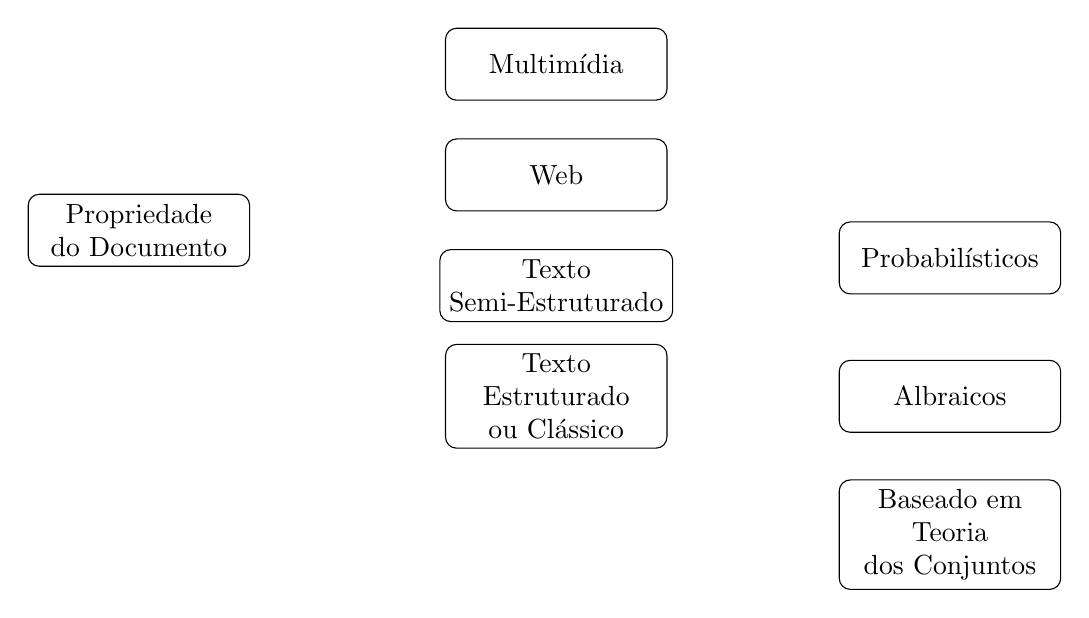
\begin{tikzpicture}[grow=right,
   level 1/.style={sibling distance=4em,level distance=5.3cm},
   level 2/.style={sibling distance=5em,level distance=5cm},
    every node/.style =
    {   shape=rectangle, rounded corners,
        draw, align=center,
        fill=white,
        minimum width = 8em,
        minimum height = 26pt,
     }  ]
\node {Propriedade \\do Documento} [grow=right]
    child {node {Texto \\ Estruturado \\ ou Clássico}
        child {node {Baseado em \\ Teoria \\ dos Conjuntos}}
        child {node {Albraicos}}
        child {node {Probabilísticos}}}
    child {node {Texto \\Semi-Estruturado}}
    child {node {Web}}
    child {node {Multimídia}};
\end{tikzpicture}
}
\caption{Taxonomia do Modelos de IR com child nodes}
\label{fig:mIRkss}
\end{figure}